\clearpage
\noindent\makebox[0pt][l]{\fontsize{13}{16}\selectfont 478}\hfill{\small\textbf{NACHLASS.}}\hfill\null\par
\vspace*{32mm}
\begin{center}
{\Large\bfseries NACHLASS.}\par\vspace{15mm}
[1.]\par\medskip
\textbf{Einfluss einer unvollkommenen Justierung am ersten Heliotrop.}
\end{center}
Der größeren Einfachheit halber nehmen wir an, dass die Achse horizontal
ist und in Richtung des Azimuts 0 zeigt, der leuchtende Punkt aber ebenfalls
am Horizont im Azimut $A$ liegt. Die Fehler sind nun doppelter Art:

\noindent I. Hinsichtlich des Azimuts.
\begin{list}{}{\setlength{\leftmargin}{9mm}\setlength{\labelwidth}{6mm}\setlength{\itemsep}{2pt}\setlength{\parsep}{0pt}\setlength{\topsep}{3pt}}
\item[1.] Wenn das Fadennetz um $\alpha$ zu weit rechts steht,
wird das Licht nicht ins Azimut 0, sondern ins Azimut
$-\alpha$ reflektiert. Also die Wirkung $=-\alpha$
\item[2.] Ist der Spiegel aus der zur Führungsstange
senkrechten Lage um $\beta$ nach vorn gedreht, so
ergibt sich daraus die Wirkung\hfill $=+2\beta$
\item[3.] Ist die Achse der Hülse zu weit von der Fernrohrachse
entfernt, im Verhältnis $(1+\gamma):1$, so ist die
Wirkung\hfill $=+206265.\gamma.\operatorname{tg}\frac12 A$
\end{list}
\noindent II. Hinsichtlich der Höhe.
\begin{list}{}{\setlength{\leftmargin}{9mm}\setlength{\labelwidth}{6mm}\setlength{\itemsep}{2pt}\setlength{\parsep}{0pt}\setlength{\topsep}{3pt}}
\item[4.] Ist der Spiegel um $\delta$ nach oben gerichtet
(die Schraube zu stark angezogen):\hfill $+2\delta\cos\frac12 A$
\item[5.] Die Spiegelachse ist unten um $\varepsilon$ zu weit
nach vorn geneigt:\hfill $+2\varepsilon\cos\frac12 A^2$
\item[6.] Die Spiegelachse steht unten um $\zeta$ zu weit rechts:\hfill $+\zeta\sin A$
\end{list}

\clearpage
\noindent\null\hfill{\small\textbf{HELIOTROP.}}\hfill\makebox[0pt][r]{\fontsize{13}{16}\selectfont 479}\par\medskip
\begin{list}{}{\setlength{\leftmargin}{9mm}\setlength{\labelwidth}{6mm}\setlength{\itemsep}{2pt}\setlength{\parsep}{0pt}\setlength{\topsep}{0pt}}
\item[7.] Die Fernrohrachse steht unten um $\eta$ zu weit nach vorn,
wobei die optische Achse dennoch zur Hauptachse
parallel werden kann:\hfill $+2\eta\sin\frac12 A^2$
\item[8.] Das Fadennetz steht um $\theta$ zu hoch:\hfill $+\theta$
\end{list}
\noindent Für das Azimut ist noch nachzutragen\par
\hspace*{9mm}Wirkung der Parallaxe $\pi$:\hfill $-\pi\sin A.$
\begin{center}\textbf{Für den zweiten Heliotrop.}\end{center}
Für das Azimut kommt nur die Neigung der beiden Spiegel zueinander in
Betracht. Ist der kleine Spiegel um $\alpha$ zu weit nach vorn gedreht, so
wird das Bild in Richtung $-2\alpha$ reflektiert.
\begin{center}
[2.]\par\medskip
\textbf{Zur Justierung des Heliotrops.}
\end{center}
1. Für die Justierung des Heliotrops braucht man vor allem zwei Stative,
von denen wenigstens eines höhenverstellbar ist und die sich mit Leichtigkeit
und Genauigkeit auf jeden erforderlichen Höhenunterschied einstellen lassen.\ .\ .\ .\ .\ .\ .

2. Der geometrische Ort des Spiegelbildes eines ruhenden Gegenstands lässt
sich, während sich der an einer Achse befestigte Spiegel um diese dreht,
am einfachsten folgendermaßen bestimmen:

Es sei $A$ der Schnittpunkt der Spiegel\textls[120]{fläche} mit der Drehachse, $B$ ein
Punkt auf der Normalen zur Spiegelfläche, und zwar auf der Rückseite des
Spiegels, und $AB$ sei beliebig gewählt. Also ist $B$ relativ zum Spiegel
fest und beschreibt bei dessen Drehung im Raum einen Kreis, und zwar im
gleichen Sinn wie irgendein anderer relativ zum Spiegel fester Punkt, z.\,B.
die Mitte einer der vier Seiten seines rechteckigen Umrisses. Zugleich liegt
der Mittelpunkt $C$ jenes Kreises auf der Drehachse, und $AC=AB\cos\theta$,
wenn $90^\circ-\theta$ die Neigung des Spiegels zur Drehachse bezeichnet.
Das Spiegelbild $P$ eines im Raum festen Punkts $D$ findet man nun, indem
man durch $D$ eine Parallele zu $AB$ zieht und sie nötigenfalls so weit
verlängert, bis $AP=AD$. Das bisher beliebige $AB$ kann man so groß wählen,
dass $AC=AE$ wird, wenn $DE$ senkrecht zur Drehachse $AE$ gezogen wird.

\clearpage
\noindent\makebox[0pt][l]{\fontsize{13}{16}\selectfont 480}\hfill{\small\textbf{NACHLASS.}}\hfill\null\par
\begin{center}
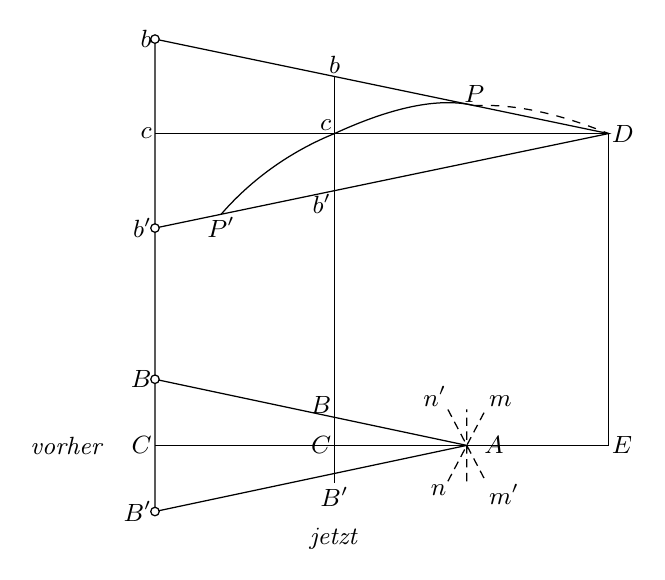
\begin{tikzpicture}[x=12mm,y=12mm,line width=.45pt,every node/.style={font=\small,inner sep=1pt}]
\draw (0,0)--(0,5)--(4.8,4)--(0,3)--cycle;
\draw (0,4)--(4.8,4)--(4.8,.7)--(0,.7);
\draw (0,1.4)--(3.3,.7)--(0,0);
\draw (1.9,4.604)--(1.9,.297);
\draw (.7,3.146) .. controls (1.05,3.55) and (1.48,3.83) .. (1.9,4) .. controls (2.40,4.23) and (2.95,4.40) .. (3.38,4.296);
\draw[dashed] (3.38,4.296) .. controls (3.9,4.32) and (4.4,4.16) .. (4.8,4);
\draw[densely dashed] (3.10,.32)--(3.50,1.08) (3.10,1.08)--(3.50,.32) (3.3,.32)--(3.3,1.08);
\foreach \q in {(0,5),(0,3),(0,1.4),(0,0)} \draw[fill=white] \q circle (.045);
\node[left] at (0,5) {$b$}; \node[left] at (0,4) {$c$};
\node[left] at (0,3) {$b'$}; \node[left] at (0,1.4) {$B$};
\node[left] at (0,.7) {$C$}; \node[left] at (0,0) {$B'$};
\node[above] at (1.9,4.604) {$b$}; \node[above left] at (1.9,4) {$c$};
\node[below left] at (1.9,3.396) {$b'$};
\node[above left] at (1.9,.997) {$B$}; \node[left] at (1.9,.7) {$C$};
\node[below] at (1.9,.297) {$B'$};
\node[above] at (3.38,4.296) {$P$}; \node[below] at (.7,3.146) {$P'$};
\node[right] at (4.8,4) {$D$}; \node[right] at (4.8,.7) {$E$};
\node[right] at (3.45,.7) {$A$};
\node[above left] at (3.12,1.08) {$n'$}; \node[above right] at (3.5,1.08) {$m$};
\node[below left] at (3.12,.32) {$n$}; \node[below right] at (3.5,.32) {$m'$};
\node[left] at (-.5,.7) {\textit{vorher}};
\node[below] at (1.9,-.14) {\textit{jetzt}};
\end{tikzpicture}
\end{center}
Zieht man dann $Dc$ parallel zu $AC$ und $Cc$ parallel zu $ED$, so ist
$Dc=2AC$, $Ac=AD$, und $c$ liegt damit auf der Oberfläche einer Kugel mit
Radius $AD$ um $A$. Legt man durch $c$ eine zu $Dc$ senkrechte Ebene und
beschreibt darin mit Radius $cb=2CB$ um $c$ einen Kreis $bb'$, so liegt
$PP'$ auf der Oberfläche des geraden Kegels mit Spitze $D$, Achse $Dc$, Seiten
$Db$, $Db'$ und Öffnungswinkel $bDb'=BAB'=2\theta$. Auf der Kugelfläche
selbst ist der Weg von $P$ zwar keine sphärische Ellipse\begingroup\renewcommand{\thefootnote}{*)}\footnote{Unter einer sphärischen Ellipse verstehe ich eine Kurve auf der Kugelfläche, von der jede Zentralprojektion eine Ellipse ist; die hier betrachtete Kurve hingegen ist eine, von der eine stereographische Projektion eine Ellipse ist.}\endgroup,\ .
unterscheidet sich aber nur sehr wenig davon. Der Durchmesser, in dessen
Verlängerung $D$ liegt, ist genau $=4\theta$; der dazu senkrechte sehr nahe
$2\theta.\frac{cD}{Ac}=4\theta.\frac{AE}{AD}$. Dieses Bild dreht sich um seinen
Mittelpunkt im gleichen Sinn wie $b$ um seinen Mittelpunkt $c$ für einen
Betrachter innerhalb des Raums $DcC$ oder wie ein Punkt $m$ oder $n$ für einen
Betrachter vor dem Spiegel. Diese Übereinstimmung des Drehsinns gilt, ob man
das Bild mit bloßem Auge oder durch ein umkehrendes Fernrohr sieht.

3. Mithilfe dieser Sätze lässt sich der kleine Spiegel nun leicht senkrecht
zur Drehachse einstellen, ob dies für die vom Fernrohr abgewandte oder für
die ihm zugewandte Lage verlangt wird.

Eine ganz grobe Annäherung, z.\,B. auf 5--10 Grad, erreicht man ohne Weiteres
nach Augenmaß. Man stelle dann das Fernrohr so ein, dass die

\clearpage
\noindent\null\hfill{\small\textbf{HELIOTROP.}}\hfill\makebox[0pt][r]{\fontsize{13}{16}\selectfont 481}\par\medskip
\noindent Spiegelachse nach Augenmaß senkrecht steht, und betrachte mit bloßem
Auge das Bild eines geeigneten Gegenstands. Wenn das Bild bei einer Drehung
des Fernrohrs nicht ruhig bleibt, muss man die senkrechte Seitenwand des
Spiegels von sich \textls[120]{abdrehen}, die sich im gleichen Sinn wie das
Bild bewegt, d.\,h. die steigende Seite, wenn das Bild steigt, die sinkende,
wenn es sinkt. Man wiederholt dies, jedes Mal von der nahezu senkrechten
Lage der Spiegelwand ausgehend, bis das bloße Auge keine Bewegung des Bildes
mehr erkennt.

Man wiederholt nun diesen Vorgang mit einem Fernrohr, das dem Spiegel
gegenüber aufgestellt wird. Ist der Fehler noch so groß, dass das Bild bei
der Drehung das Gesichtsfeld verlassen würde, muss zugleich das Fernrohr
gedreht und nötigenfalls mit seinem Stativ verschoben werden. Um im Voraus
zu beurteilen, ungefähr um wie viel und in welchem Sinn das Hilfsfernrohr
gedreht und verschoben werden muss, ist es vor allem nötig, den Sinn der
beiden möglichen Drehungen ein für alle Mal zweckmäßig zu unterscheiden.

Eine Drehung nenne ich positiv, wenn sich die Gewinde einer auf gewöhnliche
Art geschnittenen Schraube von dem auf der Schraubenachse gedachten
Betrachter entfernen. Durch eine solche Drehung schraubt man also eine
Schraube in die Mutter oder zieht die Mutter an. Bei einer Drehung um eine
senkrechte Achse, wenn der Betrachter oberhalb des gedrehten Körpers gedacht
wird, verläuft die positive Bewegung also im Sinn der täglichen Sonnenbewegung
auf der nördlichen Hemisphäre; bei einer Drehung um eine waagerechte Achse
verläuft die Bewegung in der Reihenfolge Links, Oben, Rechts, Unten: L.O.R.U,
O.R.U.L, R.U.L.O, U.L.O.R; negativ wäre L.U.R.O, U.R.O.L, R.O.L.U,
O.L.U.R.

Die allgemeine Regel ist nun folgende.

Es sei $e$ die Neigung der zum Gegenstand führenden Geraden zur Spiegelebene
und $p$ eine kleine Drehung des Fernrohrs um seine Achse (wobei der positive
Sinn von der Stellung des Betrachters vor dem Spiegel aus zu beurteilen ist,
also an der Okularseite des Heliotropfernrohrs, wenn der Spiegel dem Fernrohr
zugewandt bleiben soll, und umgekehrt im entgegengesetzten Fall). Wenn das
Bild bei dieser Drehung für das bloße Auge um $h$ \textls[120]{steigt} oder
beim Blick durch das Hilfsfernrohr um ebenso viel sinkt, muss man zur
Justierung um folgende Größe drehen
\vfill\noindent IX.\hfill61

\clearpage
\noindent\makebox[0pt][l]{\fontsize{13}{16}\selectfont 482}\hfill{\small\textbf{NACHLASS.\quad HELIOTROP.}}\hfill\null\par
\[
\frac{h}{\sin e\sin p}
\]
\[
\left.\begin{aligned}
&\text{1) der Spiegel um die Spiegelachse}\\
&\text{2) das Hilfsfernrohr ebenso weit um diese}
\end{aligned}\right\}\ \text{von oben her betrachtet.}
\]
Die letztere Bewegung erfolgt durch Drehung der Alhidade des Fernrohrs
um die Vertikalachse des Theodoliten (wenn das Hilfsfernrohr auf einem
solchen sitzt) und außerdem durch Verschiebung um
\[
\frac{h}{4\sin e\sin p}\times\delta,
\]
wenn $\delta$ den Abstand der Spiegelachse von der Theodolitenachse bezeichnet.

$h$ ist übrigens leicht zu schätzen, wenn der Radius des Gesichtsfelds
bekannt ist; beim kleinen Theodoliten ist der Durchmesser $=58'$.
In der Praxis wird eine Rechnung aber nie nötig sein; es genügt, nur den
Sinn der erforderlichen Drehungen im Voraus zu bestimmen.

4. Von den übrigen bei der Justierung des Heliotrops anfallenden Vorgängen
braucht hier nur noch derjenige erwähnt zu werden, durch den Heliotropfernrohr
und Hilfsfernrohr in eine parallele Lage mit entgegengesetzter Ausrichtung
gebracht werden. Der Abstand der Parallelen soll dem halben Abstand der
Mittelpunkte der großen Spiegel entsprechen. Früher richtete man dazu
zuerst das Heliotropfernrohr auf einen Gegenstand und legte es umgekehrt
wieder in die Lagerpfannen. Vor dem Wiedereinlegen richtete man aber das
Hilfsfernrohr in geeigneter Höhe auf denselben Gegenstand.

Jetzt ändere ich das Verfahren so ab, dass ich zuerst das Hilfsfernrohr auf
einen Gegenstand richte, dann das Heliotropfernrohr genau gegenüber, was man
daran erkennt, dass sich die Fadenkreuze mit den Bildern im jeweils anderen
Fernrohr decken. Schließlich hebe ich das Hilfsfernrohr, das auf einem
beweglichen Stativ stehen muss, um den vorgegebenen Abstand der Parallelen
an und richte es nötigenfalls, indem ich über das Heliotropfernrohr hinweg
visiere, erneut genau auf denselben Gegenstand. Ist der Gegenstand nahe, so
muss er zwei Zielpunkte bieten, deren Höhenunterschied dem vorgegebenen
Abstand entspricht; mit dem Hilfsfernrohr zielt man auf den unteren oder
den oberen Punkt, je nachdem, ob es sich in der tieferen oder höheren
Stellung befindet.
\begin{center}\rule{30mm}{.4pt}\end{center}

\clearpage
\noindent\null\hfill{\small\textbf{BEMERKUNGEN.\quad HELIOTROP.}}\hfill\makebox[0pt][r]{\fontsize{13}{16}\selectfont 483}\par
\vspace*{28mm}
\begin{center}\textbf{BEMERKUNGEN.}\end{center}
\begingroup\small
Die Notiz [1], S.~478, zur Justierung des Heliotrops ist einem Handbuch entnommen, die Notiz [2], S.~479,
die auf den 2.~Mai 1843 datiert ist, mehreren losen Blättern. Zum Heliotrop sind außer den vorstehenden Abdrucken aus den
Göttinger gelehrten Anzeigen, dem Astronomischen Jahrbuch, den Astronomischen Nachrichten und den
hier wiedergegebenen Briefen an \textsc{Olbers} und \textsc{Schumacher} auch die bereits früher abgedruckten Briefe an
\textsc{Bessel} vom 26.~Dezember 1821 und vom 15.~November 1822, an \textsc{Gerling} vom 7.~November 1822,
vom 11.~August, 1.~und 5.~September 1823 sowie die beiden Veröffentlichungen zur hannoverschen Triangulation
in den Astronomischen Nachrichten und der Bericht an das hannoversche Kabinettsministerium für 1821
(S.~349/351, 355, 381, 382/389, 397, 400 und 407/409) heranzuziehen.

Anfang Oktober 1818 hatte \textsc{Gauss} in Lüneburg gemeinsam mit \textsc{Schumacher} Anschlussbeobachtungen
an dessen südliche Dreieckspunkte durchgeführt (vgl. S.~396). Seine Beobachtungen sind in ein Tagebuch
der Sternwarte eingetragen. Bei den Messergebnissen für den Winkel Hamburg-Hohenhorn bemerkte er:

\glqq Hamburg schlecht zu sehen; das westliche, von der Sonne beleuchtete Fenster störte das Anvisieren.\grqq

Später hat \textsc{Gauss} hinzugesetzt:

\glqq N.B. Diese Erfahrung gab den ersten Anlass zur Erfindung des Heliotrops im Herbst 1820.\grqq

Von den beiden Konstruktionen des Heliotrops gab \textsc{Gauss} nach einem Brief an \textsc{Schumacher} vom
30.~März 1823 (vgl. auch den Anfang des Briefs an \textsc{Bohnenberger}, S.~364) der zweiten den Vorzug, \glqq da
ihr Gebrauch bequemer, die Justierung etwas einfacher und die größere Spiegelfläche (die sich nötigenfalls
leicht durch Abdecken verkleinern lässt) in manchen Fällen angenehm ist; auch ist der zweite Heliotrop
etwas preiswerter.\grqq\ (Letzterer kostete 125, der Heliotrop nach der ersten Bauweise 145 Taler Conv.
Münze.) Der Heliotrop der zweiten Konstruktion ist auf der Tafel S.~477 abgebildet. Eine Beschreibung
des Heliotrops der ersten und älteren Konstruktion gaben \textsc{Poggendorff} in seinen Annalen der Physik
und Chemie, Band XVII 1829, S.~83, und \textsc{Helmert} in dem Bericht über die wissenschaftlichen Apparate
auf der Londoner internationalen Ausstellung 1876, S.~169/170. Eine um ihren horizontalen Durchmesser
$AB$ drehbare Kreisscheibe trägt in ihrem Mittelpunkt $C$ eine senkrechte Achse, um die das Fernrohr
$HD$ drehbar ist. Dieses Fernrohr nimmt in einer Hülse $E$ zwischen $C$ und dem Okularende $H$ im Abstand
$CE=CA$ den Stiel $AG$ eines Spiegels $F$ auf. Der Spiegel steht senkrecht zum Stiel und dreht sich um
eine in $A$ zur Scheibe senkrechte Achse, wenn sich das Fernrohr um die Achse in $C$ dreht.
Da der Winkel $CAE=\frac12 DCA$ ist,
\par\endgroup
\begin{center}
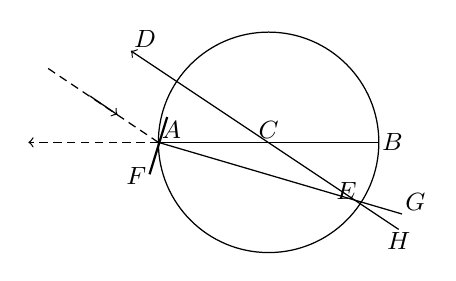
\begin{tikzpicture}[x=14mm,y=14mm,line width=.45pt,every node/.style={font=\small,inner sep=1pt}]
\draw (0,0) circle (1);
\draw (-1,0)--(1,0);
\draw[<-] (-1.25,.83)--(1.18,-.79);
\draw (-1,0)--(1.21,-.65);
\draw[line width=.8pt] (-1.08,-.29)--(-.92,.23);
\draw[densely dashed,->] (-1,0)--(-2.18,0);
\draw[densely dashed] (-2,.67)--(-1,0);
\draw[->] (-1.62,.42)--(-1.37,.25);
\node[above right] at (-1.25,.83) {$D$};
\node[above right] at (-1,0) {$A$};
\node[above] at (0,0) {$C$}; \node[right] at (1,0) {$B$};
\node[above left] at (.83,-.55) {$E$};
\node[below left] at (-1.08,-.20) {$F$};
\node[above right] at (1.21,-.65) {$G$};
\node[below] at (1.18,-.79) {$H$};
\end{tikzpicture}
\end{center}
\vfill\noindent\hfill61*

\clearpage
\noindent\makebox[0pt][l]{\fontsize{13}{16}\selectfont 484}\hfill{\small\textbf{BEMERKUNGEN.\quad HELIOTROP.}}\hfill\null\par\medskip
\begingroup\small
\noindent wird folglich, wenn das Fernrohr $HD$ auf die Sonne gerichtet ist, der Spiegel $F$ das Licht in
Richtung $CA$ reflektieren. Um den Gegenstand, dem das Licht zugesandt werden soll, in diese Richtung zu bringen,
wird das Instrument, dessen Horizontalachse $AB$ von einer Säule getragen wird, die sich auf einem Dreifuß erhebt,
so aufgestellt, dass der Gegenstand im Fernrohr $HD$ erscheint, wenn dieses zur Achse $BA$ parallel ist.
Damit der Spiegel diese Beobachtung nicht störte, war er an einem Ring befestigt.

Im Jahr 1821 hatte \textsc{Gauss} nur einen Heliotrop (vgl. S.~349 und 390), 1822 und 1823 je 3 (vgl.
S.~355 und 470), 1824 und 1825 (nach den Arbeitsberichten) je 4 Heliotrope im Gebrauch. Zu ihrer Bedienung
standen ihm neben den drei ständigen Gehilfen bei der Gradmessung (\textsc{Müller}, \textsc{Hartmann} und
\textsc{J.~Gauss}) 1824 noch zwei andere (der Student \textsc{Klüver}, den die Stadt Bremen gestellt hatte, und der Student
\textsc{Baumann}), 1825 nur ein Gehilfe (\textsc{Klüver}) zur Verfügung.
\par\hfill\textsc{Krüger.}\par\endgroup
\vspace{20mm}
\begin{center}\rule{40mm}{.4pt}\end{center}

\clearpage
\vspace*{40mm}
\begin{center}{\Large\bfseries MESSUNGSFEHLER.}\end{center}
\clearpage\null\clearpage
\vspace*{14mm}
\begin{center}
{\Large\bfseries NACHLASS UND BRIEFWECHSEL.}\par\vspace{10mm}
[Über die bei der Landestriangulation erforderlichen Instrumente.]
\end{center}
.\ .\ .\ .\ .\ .\ Bei einer ausgedehnten trigonometrischen Vermessung sind allerdings
Winkelmessinstrumente unterschiedlichen Ranges für die einzelnen Arbeiten
einzusetzen. Der Rang richtet sich nach der größeren oder geringeren
Genauigkeit, die mit dem jeweiligen Instrument zu erreichen ist. Er hängt
weniger vom Grad der Vollkommenheit der Ausarbeitung als von den Abmessungen
des Instruments ab. Dabei ließen sich viele Abstufungen vornehmen; ich
beschränke mich aber auf eine Einteilung in 3 Klassen.

Die in München gefertigten Theodoliten von 12 Zoll Durchmesser können
für die feinsten Winkelmessungen auf der Erde verwendet werden. Zum zweiten
Rang zähle ich die Repetitionstheodoliten von 8 Zoll Durchmesser aus der
\textsc{Reichenbach-Ertel}schen Werkstatt; sie dienen für sekundäre Messungen.
Für noch mehr untergeordnete Messungen sowie für Erkundungsarbeiten genügen
noch kleinere Theodoliten dritten Ranges, wobei gegebenenfalls das Repetieren
entfallen kann.

Ein Theodolit ersten Ranges \textls[120]{könnte} allerdings für \textls[120]{alle} Arbeiten
verwendet werden, auch für untergeordnete. Im Allgemeinen tut man das nicht,
teils um die größeren Instrumente zu schonen, teils weil diese von Natur aus
schwerer zu transportieren sind und ihre Aufstellung viel mehr Vorbereitungen
erfordert.

Bei den eigentlichen Gradmessungsarbeiten, die zunächst nur einen wissenschaftlichen
Zweck hatten, habe ich nur einen Theodoliten ersten und ein
